\documentclass[conference]{IEEEtran}
\IEEEoverridecommandlockouts
% The preceding line is only needed to identify funding in the first footnote. If that is unneeded, please comment it out.
\usepackage{cite}
\usepackage{amsmath,amssymb,amsfonts}
\usepackage{algorithmic}
\usepackage{graphicx}
\usepackage{textcomp}
\usepackage{xcolor}

\usepackage{url,graphicx,amsfonts,algorithm,multirow,bm,makecell,balance,subfigure,caption,color,amssymb,hyperref,cases,stfloats}
\hypersetup{
	colorlinks=true,
	linkcolor=blue,
	filecolor=blue,
	urlcolor=blue,
	citecolor=blue,
}
\def\BibTeX{{\rm B\kern-.05em{\sc i\kern-.025em b}\kern-.08em
    T\kern-.1667em\lower.7ex\hbox{E}\kern-.125emX}}
\newcommand{\tabincell}[2]{\begin{tabular}{@{}#1@{}}#2\end{tabular}}
\begin{document}

\title{PROPER\\
{\footnotesize \textsuperscript{*}a Tool for Analyzing Termination and Assertions for Affine Probabilistic Programs}
\thanks{}
}

\author{\IEEEauthorblockN{1\textsuperscript{st} Xuhui Zhao}
\IEEEauthorblockA{\textit{East China Normal University} \\
%\textit{Shanghai Key Laboratory of Trustworthy Computing}\\
Shanghai, China \\
51184501088@stu.ecun.edu.cn}
\and
\IEEEauthorblockN{2\textsuperscript{nd} Yuxin Deng}
\IEEEauthorblockA{\textit{East China Normal University} \\
%\textit{Shanghai Key Laboratory of Trustworthy Computing}\\
Shanghai, China \\
yxdeng@sei.ecnu.edu.cn}
\and
\IEEEauthorblockN{3\textsuperscript{rd} Hongfei Fu}
\IEEEauthorblockA{\textit{Shanghai Jiao Tong University} \\
Shanghai, China \\
fuhf@cs.sjtu.edu.cn}
}


\maketitle

\begin{abstract}
Probabilistic programs combine probabilistic reasoning models with Turing complete programming languages, unify formal descriptions of calculation and uncertain knowledge, and can effectively deal with complex relational models and uncertain problems. In this paper, we provide a tool for analyzing termination and assertions for affine probabilistic programs, PROPER. On one hand, it can help to analyze the termination property of affine probabilistic programs both qualitatively and quantitatively. It can check whether a probabilistic program terminates with probability 1, estimate the upper bound of expected termination time, and calculate the number of steps after which the termination probability of the given probabilistic program decreases exponentially.
On the other hand, it can estimate the correct probability interval for a given assertion to hold, which helps to analyze the influence of uncertainty of variables on the results of probabilistic programs. PROPER is demonstrated to be effective for analyzing various affine probabilistic programs.
\end{abstract}

\begin{IEEEkeywords}
Probabilistic Programming, Program Verification, Termination, Assertion Estimation 
\end{IEEEkeywords}

\section{Introduction}
In traditional logics, the representation and reasoning of knowledge is mechanical and deterministic, just like Laplace's demon, capable of inferring about the future based on the known facts. But in real world, there are a large number of uncertainty problems, which require us to use prerequisite knowledge and deductive reasoning to predict the results, that is to say, to make decisions on nondeterministic problems through probabilistic reasoning. Probability is an important tool for the representation of imprecise and incomplete knowledge. Therefore, probabilistic programs are put forward for that purpose. 

Probabilistic programs are a kind of logic programs with probabilistic facts. Probabilistic programs are often used to build generation models and reason about its hidden process. They make probabilistic reasoning models easier to build and can estimate the possibilities of certain events to occur. They can also be used to quantify the uncertainty in the prediction instead of predicting a single value. Several practical probabilistic programming languages, such as Edward~\cite{tran2016edward}, Anglican~\cite{Dav2016Design}, WebPPL~\cite{Noah2014language} and Church~\cite{Noah2012language}, can be used to build powerful models in a wide range of applications like business, military, scientific research and daily life. 
With the increasing demand for high confidence software, the analysis and verification of probabilistic programs has also received widespread attention in academia and industry. 
%Therefore, our work is a valuable and challenging, which the reliability and stability of the program can be better guaranteed. 
In general, program verification is an undecidable problem for ordinary programs.
In view of this difficulty, a realistic consideration is to verify those properties that are more important and can be verified automatically. In the current work, we present PROPER, a tool for probabilistic program verification, namely, analyzing termination and assertions for affine probabilistic programs (probabilistic programs in which arithmetic expressions are linear). The tool builds on \cite{kris2016termination,cha2015algorithmic,Sankaranarayanan2013Static}. 

Termination is an important part of  functional correctness of software. Failure to terminate a program may cause a system to become unresponsive, resulting in system failure. For termination analysis, our goal is to analyze the termination property of a given affine probabilistic program qualitatively and quantitatively. The qualitative analysis aims to answer whether an affine program terminates with probability $1$ (almost-sure termination). The quantitative analysis aims to approximate the expected termination time (expectation problem) and compute a bound $N$ such that the probability to terminate after $N$ steps decreases exponentially (concentration problem). The method we adopt is to synthesize polynomial ranking supermartingales, which is an extension of linear ranking supermartingales. 

For assertion analysis, our goal is to estimate the correct probability interval of the assertion that meets the given specifications in an affine probabilistic program. It has great potential value in artificial intelligence fields such as incomplete knowledge processing systems, meta-reasoning, cognitive query, and conformant probability planning. 
We observe that for a given probabilistic program, by selecting a finite set of appropriate paths, we can derive some facts about the behavior of the entire program. Therefore, we can use the static analysis method for probabilistic programs that can perceive, manipulate and control information based on uncertain data. For example, we first select a finite set of adequate program paths through certain strategies for estimating probability bounds. Then we evaluate each path through symbolic execution and probabilistic volumebound calculations. The sum of interval boundaries generated by each path is the probability of assertion for the program as a whole.

To summarize, this paper makes the following contributions:
\begin{enumerate}
	\item Defining and parsing probabilistic programs. More than ten kinds of probability distributions are built in, which is convenient to be called to build probabilistic models.
	\item Reducing the termination analysis of a given program to a linear programming problem. We consider the concentration results under the premise that the program is terminating. And concentration-bound analysis of probabilistic programs, which has never been implemented in other literature.
	\item Reducing the estimation of a given assertion to a polyhedron solving problem. In particular, it can handle probabilistic programs with infinitely many states.	
\end{enumerate}

Thus, as far as we know, our tool is the first implementation that can handle concentration bound of termination time, and integrate finite termination, concentration bound of termination time and probabilistic inference for affine probabilistic programs, which are the three main features for the analysis of probabilistic programs. The source code and the experimental data given in this paper are all available in the repository 
\url{https://github.com/Healing1219/PROPER}. 

\section{Preliminaries}
Probabilistic programs extend classical imperative programs by generating integer and real random values according to a fixed set of distributions. In this subsection, we illustrate the syntax and semantics of affine probabilistic programs. 

\begin{figure}[ht]
	\centering
	\begin{tabular*}{0.5\textwidth}{rcl}
		\hline
		% after \\: \hline or \cline{col1-col2} \cline{col3-col4} ...
		program\!&\!$:=$\!& typeSpecifier $\textbf{main}$ \{stmt$^*$\} \\
		stmt \!&\!$:=$\!& assign $\mid$ condStmt $\mid$ loop \\
		assign \!&\!$:=$\!& intAssign $\mid$ realAssign \\
		condStmt \!&\!$:=$\!& ifStmt $\mid$ ifElseStmt\\
		ifStmt \!&\!$:=$\!& $\textbf{if}$ LP boolExpr RP stmt$^*$\\
		ifElseStmt \!&\!$:=$\!& ifStmt $\textbf{else}$ stmt$^*$\\
		loop \!&\!$:=$\!& $\textbf{while}$ LP boolExpr RP stmt$^*$\\
		intAssign \!&\!$:=$\!&  intVar EQUAL intExpr \\
		realAssign \!&\!$:=$\!& realVar EQUAL realExpr \\
		intRandom \!&\!$:=$\!& \textbf{uniformInt}(intVar, intVar)\\
		&  & $\mid$ $\textbf{Binomial}$(intVar, realVar)\\
		&  & $\cdots$ \\
		realRandom\! &\!$:=$\!&$\textbf{uniformReal}$(realVar, realVar)\\
		&  & $\mid$ $\textbf{Gaussian}$(realVar, realVar)\\
		&  & $\cdots$ \\
		intExpr \!&\!$:=$\!&\!intConst \!$\mid$\! intRandom \!$\mid$\! intExpr\! $\pm$\! intExpr\\
		&  & $\mid$ intConst $\ast$ intExpr $\mid$ intExpr \!/\! intConst\\
		realExpr \!&\!$:=$\!&\!realConst \!\!$\mid$\!\! realRandom \!\!$\mid$\!\! realExpr \!$\pm$\! realExpr\\
		&  & \!$\mid$ \!realConst \!$\ast$\! realExpr $\mid$ realExpr \!/\! realConst\\
		boolExpr\!&\!$:=$\!& $\textbf{true}$ $\mid$ $\textbf{false}$ $\mid$ boolExpr $\wedge$ boolExpr \\
		& & $\mid$ intExpr relop intExpr \\
		& & $\mid$ realExpr relop realExpr\\
		relop \!&\!$:=$\!& $<$  $\mid$  $>$ $\mid$ $\geq$ $\mid$ $\leq$ $\mid$ $==$\\
		\hline
	\end{tabular*}
	\caption{Syntax specification of a probabilistic language}	
	\label{syntax}
\end{figure}

\paragraph{Syntax} We define a probabilistic language sufficiently expressive and easy to understand according to the syntax specification shown in Figure~\ref{syntax}. To help readability to typeset keyword and terminator in different font, bold for keyword and uppercase for terminator. The statements in the probabilistic language are similar to those in classic imperative languages, mainly composed of three types of statements: assignment, condition-branch (if/if-else) and loop(while) statements. The main difference is that we now have a collection of random value generators (discrete distribution, Binomial distribution, Poisson distribution, Integer Uniform distribution, Real Uniform distribution, Exponential distribution, Gamma distribution, Beta distribution, Geometric distribution), which can be used to simulate different probability distributions. Variables are classified into two types: program variables $X$ and sampling variables $R$. Program variables are ordinary variables that can be assigned by integer, real, boolean variables or arithmetic expressions. Boolean variables are mainly used for condition-branch and loop statements. Sampling variables are assigned with random value generators when the program is running, which is subject to a continuous or discrete probability distribution. The valuations may be different each time. Assertions is a Boolean expression over variables. In the case of compound assertions, we also support the logical operator ``and'' (\&\&) in assertion expressions.

\paragraph{Semantics} We use control flow graphs (CFGs) to express the semantics of probabilistic programs. Formally, a CFG is a tuple in the form $(L,X,R,\mapsto,\bot)$, where:
\renewcommand{\labelitemi}{$\vcenter{\hbox{\tiny$\bullet$}}$}
\begin{itemize}
	\item $L$ is a finite set of labels $L=\{\ell_0,\ell_1,\dots,\ell_n\}$ used to represent control locations. Each statement in a program has a unique label. For example, $\ell_0$ usually indicates the initial location.
	%, $\ell$$_n$ indicates the last location.
	
	\item $X=\{x_0,\dots,x_n\}$ is a set of program variables and $R=\{r_1,\dots,r_m\}$ is a set of sampling variables. When the program is running, they are assigned specific values.
	
	\item $\mapsto$ is a transition relation. Its element is in the triple form  $(\ell,\alpha,\ell')$, where $\ell$ is the current location and $\ell'$ is the next location of the transition, and $\alpha$ is the rule that must be observed 
	from $\ell$ to $\ell'$. If it is an assignment statement at the location $\ell$, $\alpha$ is an update function $\bm{f}$: $\mathbb{R}^{X\cup R}\to \mathbb{R}^{X}$. In the other case, if it is a condition-branch or loop statement at the location $\ell$, $\alpha$ is a propositional polynomial predicate.
	
	\item $\bot$ is a special label not in $L$, or it can be written as $\ell_\bot$, which  means the termination of the program.
\end{itemize}

Obviously, any probabilistic program can be transformed into a CFG naturally. Each label represents the control location in the execution of the probabilistic program, as shown in Figure~\ref{example1}. 
We assume that a probabilistic program $P$ has two sets $X=\{x_0,\dots,x_{n}\}$ and $R=\{r_0,\dots,r_{m}\}$, and use $v_x$ and $v_r$ to represent the set of all valuations on $X$ and $R$, respectively. The valuation over variables is a series of functions $\bm{f}$: $v_{x_{i+1}}=f_i(v_{x_{i}}, v_r)$.  
Let $(L,X,R,\mapsto,\bot)$ be the CFG associated with the probabilistic program $P$. For notational convenience we assume the configuration is a tuple $(\ell, v_x)$, where $\ell$ is a location of $P$ and $v_x$ is a valuation of variables.
We fix $(\ell_0, v_{x_0})$ to be the initial configuration of the program $P$. The program updates its state according to the transition relation. The transition relation $(\ell,\alpha,\ell')$ specifies the transitions between labels together with the transition rules $\alpha$ specific to different types of labels.
The execution of $P$ is an infinite sequence of configurations with each prefix in the form $(\ell_0, v_{x_0}) \dots (\ell_k, v_{x_k})$. By convention, we assume that when a program terminates, it stays in the terminal location $\bot$ forever, so that terminating executions are also infinite. 
For each $0\leq i\leq k$ in the configuration sequence $(\ell_0,v_{x_0}) \cdots (\ell_k, v_{x_k})$, an execution enables the transition relation $(\ell_i, \alpha, \ell_{i+1})$ in $(\ell_i, v_{x_i})$, and evaluates the random variable $v_r$ so that $v_{x_{i+1}}=f_i(v_{x_i},v_r)$. If there is a finite path starting from $(\ell_0, v_{x_0})$ and ending with $(\ell_k, v_{x_k})$, we can access the configuration $(\ell_k, v_{x_k})$ from the starting configuration $(\ell_0, v_{x_0})$. 

Suppose the current configuration is $(\ell_i, v_{x_i})$. According to different types of statements, the transition relation of each label can be divided into the following cases. 
\renewcommand{\labelitemi}{$\vcenter{\hbox{\tiny$\bullet$}}$}
\begin{itemize}
	\item  Assignment statements: $x:=exp$, where $x$ is a variable and $exp$ is a constant or arithmetic expression or function reference. According to the transition relation $(\ell, \alpha, \ell_{i+1})$, $\alpha$ is an update function $f$: $\mathbb{R}^{X\cup R}\to \mathbb{R}^{X}$, the configuration of $P$ changes into $(\ell_{i+1}, v_{x_{i+1}})$, where $v_{x_{i+1}} = f_i(v_{x_{i}},v_r)$.
	
	\item  Conditional-branch statements: $\textbf{if}$  $\alpha$  $\ell_a$ $\textbf{else}$ $\ell_b$. If the value of $\alpha$ is true ($v_{x_i} \models \alpha$), the configuration of $P$ changes into $(\ell_a, v_{x_i})$. Otherwise, it changes into $(\ell_b, v_{x_i})$.
	
	\item  Loop statements: $\textbf{while}$ $\alpha$ \{$\ell_{i+1}$\}. If the value of $\alpha$ is true ($v_{x_i} \models \alpha$), the configuration of $P$ changes into $(\ell_{i+1}, v_{x_i})$. Otherwise, it changes into $(\bot, v_{x_i})$, where $\bot$ means the exit of the loop.
	
	\item  Location of termination: $\ell_{i+1} =\ell_{i}=\bot$, which marks the end of $P$, and in this case $v_{x_{i+1}} = v_{x_i}$.
\end{itemize}

\begin{figure}[htbp]
	\vspace{-0.1cm}  %调整图片与上文的垂直距离
	\centering %居中
	\subfigure{ %第一张子图
		\begin{minipage}{3.5cm}
			\centering %子图居中
			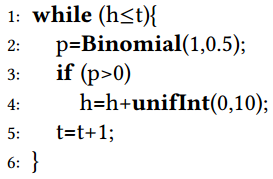
\includegraphics[scale=0.85]{img/ex1} 
		\end{minipage}
	}
	\subfigure{ %第二张子图
		\begin{minipage}{6.5cm}
			\centering %子图居中
			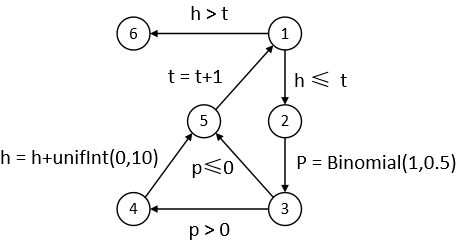
\includegraphics[scale=0.9]{img/CFG1} 
		\end{minipage}
	}
	\caption{A probabilistic program with its CFG} % %大图名称
	\label{example1} %图片引用标记
	%\setlength{\belowcaptionskip}{-3cm}   %调整图片标题与下文距离
\end{figure}

\textbf{Example 1.} In Figure~\ref{example1}, we show a probabilistic program on the top and its control flow graph on the bottom. In the program,  $t, p$ and $h$ is a program variable, Binomial(1,0.5) and unifInt(0,10) are sampling variables. Binomial(1,0.5) represents a binomial distribution, the first parameter represents the number of experiments and the second parameter represents the probability of success, which yields values 0 and 1 with equal probability; unifInt(0,10) represents an integer uniform distribution, which yields the integers between 0 and 10  with equal probability. The numbers 1-6 on the left are the program control locations, the initialization of $h$ and $t$ is omitted at location 0. The probabilistic program simulates a scene of the tortoise hare race. The tortoise's initial position is $t$ and the hare's initial position is $h$.  The tortoise  always moves at the speed of 1. When $p>0$, that is to say, there is a probability of 0.5, the hare increases its speed by a random number between 0 and 10. The program terminates when the hare passes the tortoise.

\section{Termination Analysis}
Termination analysis is an important part of program verification. If a loop program terminates for all initial values that can enter the loop, the program is said to be terminating. Ensuring termination is a necessary condition for many properties of programs such as total correctness. 

Generally speaking, the termination of a program is undecidable, but for some subclasses of programs, the termination can be verified. In this paper, we first extend the traditional linear ranking supermartingale to polynomial ranking supermartingales~\cite{Chakarov2013Martingales}, and verify the termination of affine probabilistic programs by synthesizing polynomial ranking supermartingales. PROPER implements Algorithm \ref{TA}~\cite{kris2016termination,cha2015algorithmic} to analyze probabilistic termination qualitatively and quantitatively.  

\paragraph{Qualitative analysis} It mainly analyzes whether a probabilistic program will terminate with probability $1$ (almost sure termination).
Let us recall the concepts of invariant, pre-expectation, and polynomial ranking supermartingale.

 \textbf{Invariant} is a function $I(\ell)$ that assigns a propositional polynomial predicate on variables $X$ to each label $\ell$. Thus for all configurations $(\ell,v_x)$  reachable from the initial configurations $(\ell_0, v_{x_0})$ by running the program, it will hold that $v_x \vDash I(\ell)$. In PROPER, we only support linear invariants, and every $I(\ell)$ is a finite union of polyhedra.
 
 \textbf{Example 2.} We consider the same program as in Example~1 with the CFG in Figure~\ref{example1}. We assign the trivial invariant $I$ such that $I(1)=h\leq t+9$,$I(j)=h\leq t$ for $j=2,3$,$I(4)=h\leq t \land p\ge 0$,$I(5)=h\leq t+10$ and $I(\bot)=t\le h$.
 
 \textbf{Pre-expectation} is intuitively the expected value of the polynomial ranking  supermartingale $g(\ell, v_x)$ in the next step of program execution. We define it as the function $pre_g(\ell, v_x)$, as follows:

\begin{numcases}{pre_g(\ell,v_x)=}
	\mathbb{E}(g(\ell',f(v_x,v_r)),\label{assign}\\
	\boldsymbol{1}_{v_x\vDash\alpha} \cdot g(\ell_a,v_x)+\boldsymbol{1}_{v_x\nvDash\alpha} \cdot g(\ell_b,v_x), \label{condition} \\
	g(\ell,v_x), \label{terminal}
\end{numcases}

 Equation \eqref{assign} is for assignment statement. $\ell'$ is the next location and $f(v_x,v_r)$ is a update function. The expectation is about $v_r$, which is a random variable following its cumulative distribution function, and $\ell'$ and $v_x$ are regarded as constants.  
 Equation \eqref{condition} is for condition(if/if-else) or loop(while) statement. When $v_x \vDash\alpha$, it means that $\boldsymbol{1}_{v_x\vDash\alpha}$ is equal to 1, otherwise, it is equal to 0. Similarly, $\boldsymbol{1}_{v_x\nvDash\alpha}$ is opposite to the above situation. $\ell_a$ and $\ell_b$ are the labels for \textbf{true}-branch($v_x\vDash\alpha$) and \textbf{false}-branch($v_x\nvDash\alpha$) respectively. 
 Equation \eqref{terminal} is for terminal statement, that is $\ell$ is at $\bot$ location.
 
 \textbf{Polynomial ranking supermartingale}~\cite{Chakarov2013Martingales} (pRSM) is intuitively a polynomial with the maximal degree $d$ at each location. At the same location, the pre-expectation does not exceed the value of pRSM. Each pRSM function is non-negative at a non-terminal location, and the dividing line between termination and non-termination is 0.
 
\textbf{Example 3.} We consider again the same program as in Example~1. We assume the maximal degree of the pRSM template as $2$. The quadratic template $g(\ell, v_x)$ is shown in the following formula, where $n=1,\ldots,5$. 
\begin{align*}%加*表示不对公式编号
\begin{split}
g(\ell_n,h,t,p)=&a_{n_0}+a_{n_1}\!\cdot \!h+a_{n_2}\!\cdot \!h^{2}+a_{n_3}\cdot \!ht +a_{n_4}\cdot \!hp+\\
&a_{n_5}\cdot\! t +a_{n_6}\cdot\! t^{2}+a_{n_7}\cdot\! tp+a_{n_8}\cdot\! p+a_{n_9}\cdot\! p^{2}
\end{split}
\end{align*}
Then we can calculate the pre-expectation, where all the coefficients involved are linear w.r.t. $a_{n_i}$.\\ For the assignment statement at location $\ell_2$:
 \begin{align*}
 \begin{split}
 pre_g(\ell_2,h,t,p)&=\mathbb{E}(g(\ell_3,h,t,p)) \\
 &=\!(a_{30}\!+0.25a_{39}\!+0.5a_{38}\!)\!+\!(a_{31}\!+\!0.5a_{34})\cdot \!h+ \\
 &\quad a_{32}\cdot \!h^{2}\!+\!a_{33}\cdot ht\!+(a_{35}\!+\!0.5a_{37})\cdot t\!+a_{36}\cdot t^{2}  
 \end{split}
 \end{align*}
 For the condition statement at location $\ell_3$, if the condition $p>0$ holds:
 \begin{align*}
 \begin{split}
 pre_g(\!\ell_3,h,t,p\!)&\!=g(\ell_4,h+unifInt(0,10),t,p) \\
 &\!=\!(a_{40}\!+\!5.5a_{41}\!+\!0.25a_{42})\!+\!(a_{41}\!+\!11a_{42})\!\cdot\! h+ \\
 &\quad\!a_{42}\!\cdot\! h^{2}\!+\!a_{43}\!\cdot\!ht\!+\!a_{44}\!\cdot\! hp+(5.5a_{43}\!+\!a_{45})\!\cdot\! t \\
 &\quad\!+\! a_{46}\!\cdot\! t^{2}\!+\!a_{47}\!\cdot\! tp +(a_{48}\!+\!5.5a_{44})\!\cdot\! p\!+\!a_{49}\!\cdot\! p^{2} 
 \end{split}
 \end{align*}
 Otherwise, its next location is $\ell_5$:
 \begin{align*}
 \begin{split}
 pre_g(\ell_3,h,t,p)&=g(\ell_5,h,t+1,p) \\
 &\!=\!(a_{50}\!+\!a_{55}\!+\!a_{56})\!+\!(a_{51}\!+\!a_{53})\cdot h\!+\!a_{52}\cdot h^{2}+\\
 &\quad a_{53}\cdot ht\!+a_{54}\cdot hp\!+(a_{55}+2a_{56})\!\cdot\! t\!+\!a_{56}\cdot t^{2} \\
 &\quad +a_{57}\cdot tp+(a_{57}+a_{58})\cdot p+a_{59}\cdot p^{2}
 \end{split}
 \end{align*}
 
 Assuming the invariant is represented by $I$, the polyonomial ranking-supermartingale map \textit{w.r.t} $(P,I)$ meets the following conditions.
 \begin{itemize}
 	\item C1: For each location $\ell$, $g(\ell,v_x)$ is a polynomial over program variables of order at most $d$;
 	\item C2: For non-terminal location and reachable
 	valuations $v_x \vDash I(\ell)$, we have $g(\ell,v_x) \geq 0$;
 	\item C3: For terminal location, $g(\ell,v_x)=K$;
 	\item C4: For non-terminal location and reachable
 	valuations $v_x \vDash I(\ell)$, we have $pre_g(\ell,v_x) \leq g(\ell,v_x)-\epsilon$.
 \end{itemize}
 In the above formula, $\epsilon \geq 0$ and $K \leq -\epsilon$. C1 is the polynomial condition; C2 is the non-termination condition, which shows that the pRSM is non-negative for every non-terminal location; C3 is the termination condition, which specifes that pRSM should always be less than 0 at terminal location; C4 is the RSM difference condition, which specifies that at all reachable configurations $(\ell, v_x)$, the pre-expectation is no more than the difference between the pRSM and $\epsilon$. From the above four conditions, it can be seen that $g(\ell,v_x) \geq K$, where $K$ is a lower bound, so this method cannot handle distributions without lower bounds, such as Gaussian distributions.
 
  \textbf{Example 4.} Consider again Example~1 with invariant given in Example~2 and pre-expectation given in Example~3, we can list the equation for the termination of the program as follows:
 \begin{itemize}
 	\item[-] (C4, label 1): $g(\ell_2,h,t,p)\leq g(\ell_1,h,t,p)-\epsilon$
 	\item[-] (C4, label 2): $\mathbb{E}(g(\ell_3,h,t,Binomial(1,0.5))) \leq g(\ell_2,h,t,p)-\epsilon$;
 	\item[-] (C4, label 3): $g(\ell_4,h,t,1) \leq g(\ell_3,h,t,p)-\epsilon$ and $g(\ell_5,h,t,0) \leq g(\ell_3,h,t,p)-\epsilon$;
 	\item[-] (C4, label 4): $ p\},\mathbb{E}(g(\ell_5,h+unifInt(0,10),t,p)) \leq g(\ell_4,h,t,p)-\epsilon$;
 	\item[-] (C4, label 5): $g(\ell_1,h,t+1,p)\leq g(\ell_5,h,t,p)-\epsilon$;
 	\item[-] (C2): $g(\ell_i,h,t,p) \geq 0$ for $1\leq i \leq 5$.
 \end{itemize}

 We have observed that each of the universal quantization formulas described in C2 and C4 can be decomposed into a conjunction. This decomposition process can be solved by quantifier elimination, but this method requires strong computing power. In order to reduce the cost, we rely on Handelman's Theorem~\cite{Handelman1988}, which uses positive linear functions to represent polynomials on compact convex polyhedra.
 
 In the following, we present some basic definitions about Handelman's Theorem. Let $\Gamma$ be a finite set of linear functions (polynomials of degree 1) over $X$, which is a finite set of variables. The monoid of $\Gamma$ is defined as
 
 $$Monoid(\Gamma):=\Big\{\prod_{i=1}^{n} g_i|n\in\mathbb{N}_0\quad and \quad g_i,\dots g_n\in\Gamma\Big\}.$$
 
 \textbf{Handelman's Theorem.} Let $h \in \mathbb{R}[X]$ be a polynomial such that $g(x) \ge 0$ for all $x \in \{\Gamma\}$. If $\{\Gamma\}$ is compact, then
 $$h = \sum_{i=1}^{m}c_i\cdot f_i$$
 for some $m \in \mathbb{N}$, $c_1,\dots,c_m\ge 0$ and $f_1,\dots,f_m\in Monoid(\Gamma)$.
 
 Handelman's theorem requires that every polynomial $g$ must be a positive linear combination of polynomials in $Monoid(\Gamma)$. By definition, $c_i$ is a set of non-negative real coefficients, $f_i\in Monoid(\Gamma)$. For every $X\in \Gamma$, we can construct $g(X) \ge 0$ over invariants $I(\ell)$. In PROPER, we fix a natural number $n$ such taht the element in $Monoid(\Gamma)$ are multiplied by at most $n$ elements.
 
 According to Example~3, the forms of $pre_g(\ell,v_x)$ and $g(\ell)$ are known. Then according to the pRSM(C4), we can symbolically calculate the polynomial $H=g(\ell, v_x)-pre_g(\ell,v_x)-\epsilon$ for each location $\ell$. According to Example~2, we know the invariant $I(\ell)$, which is used as the set $\Gamma$ of linear functions. We use $H'$ to express the polynomial about Handelman's theorem.
 Coincidentally, the coefficients $a_{ni}$ of $H$ and $c_m$ of $H'$ match exactly. Finally, it is transformed into a linear programming problem. 
 A solution of the linear equations ensures that the probabilistic program can terminate almost surely.
  
\begin{algorithm}[htb]  
	\caption{Termination Analysis.}  
	\label{TA}  
	\begin{algorithmic}[1]  
		\REQUIRE 
		Program $P$; 
		\ENSURE  
		Judge whether the program is terminating, isT;\\
		The probability to terminate after $N$ steps decreases exponentially, $N$.
		\STATE Set template $g(\ell,v_x)$ with a natural number as the maximal degree. Each location has the common template with unique coefficient. If $\bot$, the template $g(\ell,v_x)$=$K$.
		\STATE Traverse the abstract syntax tree \\
		2.1: Calculate the invariant $I(\ell)$ for each location.\\
		2.2: Calculate the pre-expectation for each location.\\
		\STATE  Construct polynomials. $H=g(\ell,v_x)-pre_g(\ell,v_x)-\epsilon$, where $\epsilon >0$ and $K \leq -\epsilon$
		\STATE Handelman's Theorem. $H'=\sum\limits_{i=1}^{m} c_i \cdot f_i$, where $f_i \in Monoid(\Gamma)$, $Monoid(\Gamma)=\{\prod\limits_{i=1}^{n} I(\ell_i) | n\in\mathbb{N}_0$ and $ I(\ell_1),\dots,I(\ell_n) \in I\}$ and $c_i$ is a non-negative real number.
		\STATE Solve linear programming. $H$ and $H'$ are corresponding coefficients match exactly. If solvable, the program $P$ can be terminating, and can continue with step 6, otherwise return.
		\STATE Calculate the upper bound of expected termination time according to $ET(P)\leq UB(P):=\frac{g(\ell_0,v_0)-K}{\epsilon}$
		\STATE Calculate the difference interval $[a,b]$ satisfying the condition $a\leq g(\ell',f(v_x,v_r))-g(\ell,v_x)\leq b$
		\STATE Obtain $N$, according to $\mathbb{P}(T_p > N) \leq e^{-\frac{2(\epsilon(N-1)-g(\ell_0,v_0))^2}{(N-1)(b-a)^2}}$
	\end{algorithmic}  
\end{algorithm} 

Termination analysis qualitatively has five steps, let us consider Step 1 to 5 in Algorithm \ref{TA}. Theoretically, template $g(\ell,v_x)$ can be a polynomial of any positive integer  degree. For the sake of simplicity, in PROPER, we take the maximal degree of the template as 2. 
Then we can calculate invariants and pre-expectation by traversing the abstract syntax tree. Evidently, if $g(\ell,v_x)$ is a polynomial on program variables and it is an assignment(ref. Equation \eqref{assign}), condition-branch or loop statement(ref. Equation \eqref{condition}) at location $\ell$, then the pre-expectation is also a polynomial. 
When $\ell$ is at the terminal location(ref. Equation (\ref{terminal})),  $pre_g(\ell,v_x)$ is equal to $g(\ell,v_x)$, that is, the value of $pre_g(\ell,v_x)$ is negative number $K$(ref. C3).
The next step is to construct polynomials $H$(ref. C4) with known $pre_g(\ell,v_x)$ and $g(\ell,v_x)$. Then we construct polynomials $H'$ by using Handelman's theorem and invariant $I(\ell)$ which we have worked out in the step 2.1.
The last step is to compute  the coefficients of template $g(\ell,v_x)$. If there is a solution indicating the existence of pRSM, the probabilistic program will terminate with probability 1(almost sure termination).

Back to Example~1, assuming that the initial value of h is 5 and t is 30, it obviously satisfies the condition $h \leq t$. In addition, $\epsilon$ is taken as $1$ and $K$ as $-1$ for our tool PROPER. Below we show the result of Example 1 in Table \ref{RSM}.

\begin{table}[htb]
	\centering
	\caption{The RSM for Example 1}
	\label{RSM}
	\begin{tabular}{|c|c|c|}
		\hline
		Label& Invariant & The RSM-map  \\ \hline
		1 & $h\leq t+9$ &$3\cdot t-3\cdot h+27$ \\ \hline
		2 & $h\leq t$ &$3\cdot t-3\cdot h+26$ \\ \hline
		3 & $h\leq t$  &$3\cdot t-3\cdot h-14\cdot p+32$ \\ \hline
		4 & $h\leq t\land p=1$ &$3\cdot t-3\cdot h+17$ \\ \hline
		5 & $h\leq t+10$&$3\cdot t-3\cdot h+31$ \\ \hline
		6 & $t<h$ &$-1$ \\ \hline
	\end{tabular}
\end{table}

The ``Label" column lists control locations of the program. The ``Invariant" column gives the logical formulas that the reachable labelled locations satisfy when the program is executed from the starting location. The ``The RSM-map" column denotes the ranking supermartingale on the labels. The expected value of the RSM decreases by at least a positive amount $\epsilon$ after each execution of a statement. We can see that, when going from label 1 to label 2, the expected value of the supermartingale decreases by 1. Similarly  in the step from label 2 to label 3,  the condition is met because $p=\mathbb{E}(Binomial(1,0.5))=0.5$. And when the ``while" condition is not met, the expected value is $K$.

\paragraph{Quantitative analysis} We aim to estimate the upper bound of expected termination time and calculate the bound $N$, so that the probabilistic program concentrates on termination before $N$ steps. 

We focus on the approximation of the expected termination time, as given in Steps 6 to 8 in Algorithm \ref{TA}. According to the previous steps, we can find the coefficients of the polynomial template pRSM. The existence of a pRSM ensures a finite upper bound on the expected termination time. If we know the initial values of variables, we can see that the value at the first location is $g(\ell_0, v_0)$, the value is $K$ at the terminated location $\ell_\bot$ and the difference between two consecutive locations is $\epsilon$.  Therefore, when program $P$ is almost surely terminating, we can get the upper bound on termination time for the given initial condition: $ET(P) \leq UB(P) = \frac{g(\ell, v_0)-K}{\epsilon}$. 

Then we focus on the concentration problem, that is, the probability of termination after $N$ steps shows an exponential decrement. Exponential sum is one of the most commonly used specific function families in nonlinear approximation theory. Our main idea is based on martingale inequality of Azuma's Inequality~\cite{Azuma1967}, Hoeffding's Inequality~\cite{Hoeffding1963,McDiarmid1998Concentration}  and Bernstein's Inequality~\cite{Bennett1962,McDiarmid1998Concentration}. In probability theory, the Azuma's inequality gives a concentration result for the values of martingales that have bounded differences. Hoeffding's Inequality is a special case of Azuma's Inequality. It proposes an upper bound on the probability that the sum of random variables deviates from its expected value. Bernstein's Inequality is a generalization of Hoeffding. It can handle not only independent variables but also weak independent variables. By Chatterjee~\emph{et al.}~\cite{cha2015algorithmic}, we know that if $\epsilon(N-1) > g(\ell_0,v_0)$, the inequality $\mathbb{P}(T_p > N)\leq e^{-\frac{2((N-1)-g(\ell_0,v_0))^2}{(N-1)(b-a)^2}}$ holds. 

\textbf{Example 4} Consider again Example 1 with the initial values t=30 and h=5. We have  $ET(P) \leq \frac{3\cdot 30-3\cdot 5+27-K}{\epsilon}=103$, where $K$ and $\epsilon$ are set to be -1 and 1, respectively. The difference interval exists, which is [-28,14]. Suppose we make the query $\mathbb{P}(T_p > N)\leq 10^{-3}$, the number $N$ can be computed to be 6296  approximately.

\section{Estimating the probabilities of assertions}
The goal of this section is to estimate the probability that a given assertion is correct at the exit of a program. For the specific algorithm, we refer to~Sankaranarayanan~\emph{et al.}~\cite{Sankaranarayanan2013Static}. There are two main steps.

The first step is to generate a sufficient and appropriate path set $S$ with high confidence coverage. The finite set $S=\{s_1,\dots,s_i,\dots,s_n\}$ contains distinct paths that are terminating, where $s_i$ is the transition sequences $\ell_0 \to \dots \to \ell_k \to \dots \to \ell_\bot$. An infinite number of paths may be generated by the control flow of loop statements over program variables and sampling variables. Therefore, the symbolic execution~\cite{Geldenhuys2012symbolic} method is adopted to collect path sets. It can improve the coverage of path set $S$ to all paths in a limited time. Without requiring specific input, symbolic execution can systematically explore as many unique execution paths as possible, ensuring high coverage. All execution paths of a program can be expressed as a tree, called an execution tree, as shown in Figure \ref{executionTree}. Each execution state, represented by a box, shows the statement to be executed. In the upper row of the box, $X$ represents a symbol storage that associates variables with a specific value or an expression on the symbolic value $x_i$. And $\pi$ respresents path constraints, that is, a formula representing a set of hypotheses on the symbol $x_i$ due to the branch taken during execution to reach $stmt$. At the beginning, $\pi=true$. Both $X$ and $\pi$ are updated during the symbolic execution. In the bottom row of the box, $stmt$ is the next statement to be evaluated, it can be an assignment, condition-branch or loop statement.

\begin{figure}[h]
	\centering
	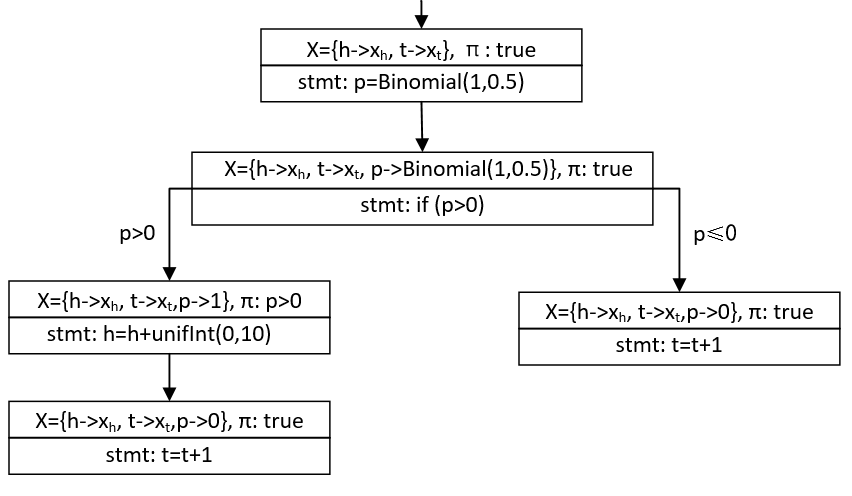
\includegraphics[scale=0.6]{img/executionTree}
	\caption{Symbolic execution tree for Example 1}
	\label{executionTree}
\end{figure}

Through a symbolic execution, we traverse the program execution tree and collect the symbolic states and path constraints, so that each path of the program execution is based on the original probability distribution. At the same time, we also do some simplification work to avoid interference from irrelevant steps. For example, if there is a condition-branch, but neither the if-branch nor the else-branch will affect the variables related to the assertion, then the condition-branch belongs to the irrelevant setp.
Suppose the set of paths $S$ has a lower bound $c$ on their combined path probabilities. We can still consider the estimated probability of a given assertion $\varphi$ on path set $S$ as an approximation over the whole program, and know that the contribution from the unexplored path is at most $1-c$. In this way, our method is able to handle the problem that program $P$ contains program variables and sampling variables with a wide range of distributions or even infinitely many states. 

The second step is path probability bound computation and estimating the probability of a given assertion. 
For the path set $S$ collected above, we can analyze each path in turn, then estimate the path probability $c$. Each path has a series of variables and constraints. Given the probability distribution on variables, we need to estimate the probability of satisfying all constraints. In an overall view, it boils down to finding the satisfaction probability of the constrained system when the probability distribution of a single variable is given. Similar to calculating path probabilities, we can estimate the probabilities of assertions over variables by providing guaranteed interval bounds on assertion probabilities. The path condition is a conjunction of linear inequalities, so it is a convex polyhedron on $R$. Each variable can be regarded as a dimension of convex polyhedron.
Since the calculation of the accurate probabilities is closely related to the volume of $n$-dimensional convex polyhedron, when the dimension increases, the calculation becomes very difficult and the time complexity is high~\cite{Arora1998Proof}. Usually, the computation may fail due to the calculation or insufficient memory. 
On the premise of weighing the efficiency and accuracy of calculation, we focus on calculating lower and upper bounds of a given assertion rather than the estimated value. 

\begin{algorithm}	
	\caption{mcBoundProbability}	
	\label{mcBoundProbability}	
	\begin{algorithmic}[1]	
		\REQUIRE Polytop p=(vars, constraints), maxDepth		
		\ENSURE Probability interval $[p_1, p_2]$		
		\IF{$isABox() || maxDepth<=0$}		
		\STATE $[p1,p2]+=computeBoundingProbability()$;	
		\ENDIF  \\		
		$//$ If at least two (or more) non trivial clusters remain, then perform the decomposition.  		
		\IF{$isDecomposable(p)$}		
		\STATE dim = $selectBranchDimension()$;		
		\STATE branches= $branchAndBound(dim, nBranch)$;		
		\FOR{$b$ in branches}		
		\STATE $mcBoundProbability(b, maxDepth-1)$;		
		\ENDFOR
		\ENDIF
	\end{algorithmic}
\end{algorithm}

\begin{figure*}[htbp]
	\centering
	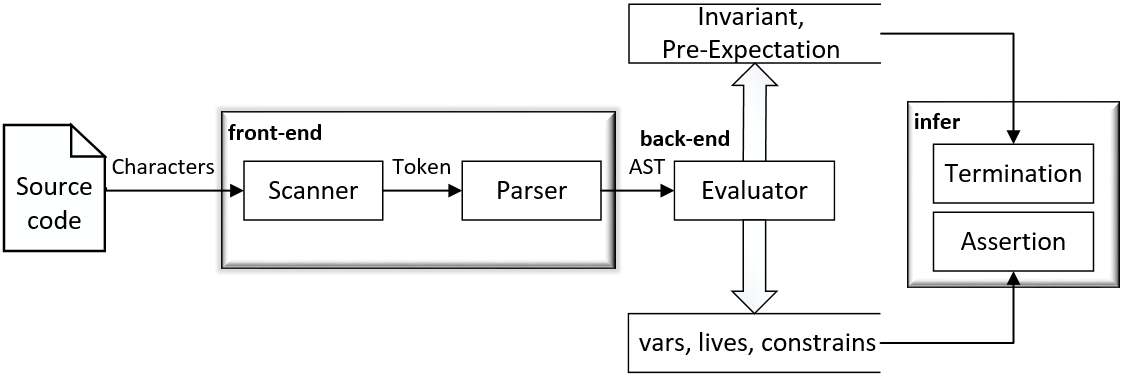
\includegraphics[scale=0.6]{img/architecture}
	\caption{The architecture of PROPER}
	\label{architecture}
\end{figure*}

The calculation of path probabilities can be reduced to a polyhedron solving problem~\cite{Visser2012Green}. However, the solution of a convex polyhedron by linear programming is too rough. Therefore, we first decompose the convex polyhedron into several non-intersecting convex bodies~\cite{Bingsheng2020} and then add up the calculation results, as described in Algorithm~\ref{mcBoundProbability}. The input to the algorithm is $maxDepth$ and a polytop structure composed of variables and constraints. The $maxDepth$ is the maximum recurrence depth, in order to avoid infinite decomposition, with the default value $12$ in PROPER. The output is the upper bound and the lower bound of the probability. The function $isABox()$ returns true if each dimension is bounded. The function $isDecomposable()$ is used to determine whether the current dimension can be decomposed. The function $selectBranchDimension()$ is based on the idea of importance sampling, selecting an unbounded or semi-bounded dimension or else it will select the maximum width dimension. The function $branchAndBound()$  performs the decomposition according to the selected dimension. Here, $nBranch$ is the number of segmentation, with the default value $2$. The function $computeBoundingProbability()$ is used to calculate the upper and lower bounds. 

The general idea of Algorithm~\ref{mcBoundProbability} is to use multiple hypercubes to approximate a given polyhedron. The boundary of hypercube is found by continuously selecting the most influential dimension and decomposing along the selected dimension. When the boundary box is found or the maximum recursion depth exceeds $maxDepth$, the upper and lower bounds will be calculated.
The paths in the set $S$ are calculated in turn. Since there is no intersection of each path, the path probability is equal to the sum of each paths' probability. The method of calculating the assertion probability is the same as above. The assertion can be regarded as a set of constraints. Therefore, the constraint is equivalent to the disjunctive normal form of path constraint and assertion.
Let us assume that the calculation result of path probability is $[p_1,p_2]$ and assertion probability is $[p_{1'},p_{2'}]$. It indicates that the maximum $(1-p_1)$ path has not been explored. The upper bound of the assertion probability needs to be corrected by adding $(1-p_1)$. Therefore, the ultimate probability of satisfying the assertion is in the interval $[p_{1'},p_{2'}-p_1+1]$.

\section{Implementation and Experimental Evaluationn}
PROPER's architecture is mainly composed of three parts: a front-end, a back-end and an inference engine, as shown in Figure \ref{architecture}.  

The front-end and back-end can be regarded as a whole, based on an interpreter, which converts the source code into some effective intermediate representations and executes them line by line. The front-end is similar to a usual compiler front-end, including a scanner and a parser. The scanner performs lexical analysis by converting the  source code  into a token stream.  The output of the scanner is used as the input of the parser to construct an abstract syntax tree.
%In this process, a symbol table is created. It is essentially a database to store related information such as variables and function calls. We use a hash table to implement the symbol table, which helps to quickly and effectively insert new data nodes, access and update existing data nodes. 

\begin{figure*}[hb]
	%\vspace{-0.5cm}  %调整图片与上文的垂直距离
	\centering %居中
	\subfigure[For termination analysis]{ %第一张子图
		%\begin{minipage}{5cm}
		\centering %子图居中
		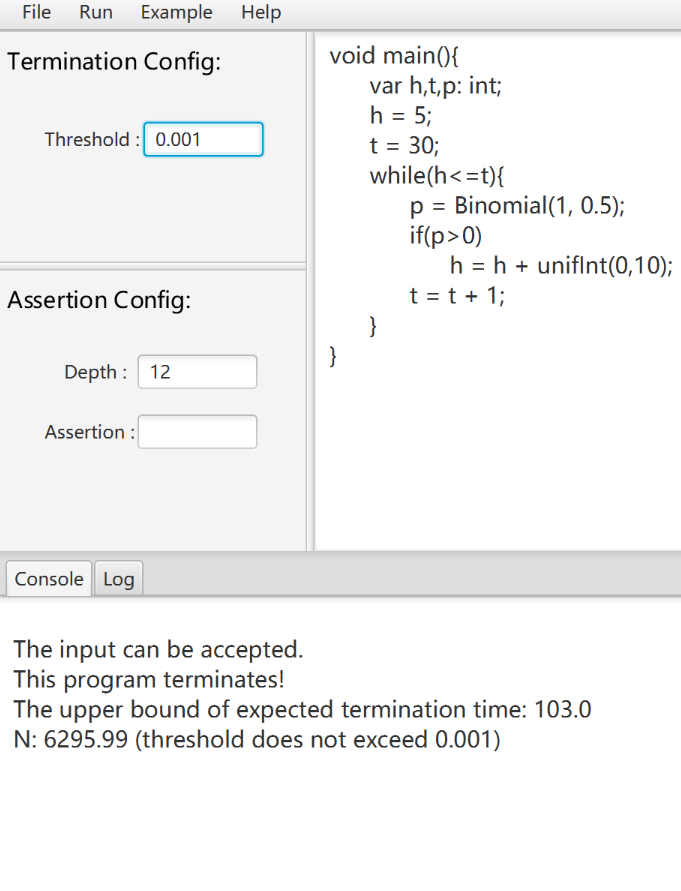
\includegraphics[scale=0.65]{img/interface1} 
		%\end{minipage}
	}\hfill
	\subfigure[For assertions analysis]{ %第二张子图
		%\begin{minipage}5cm}
		\centering %子图居中
		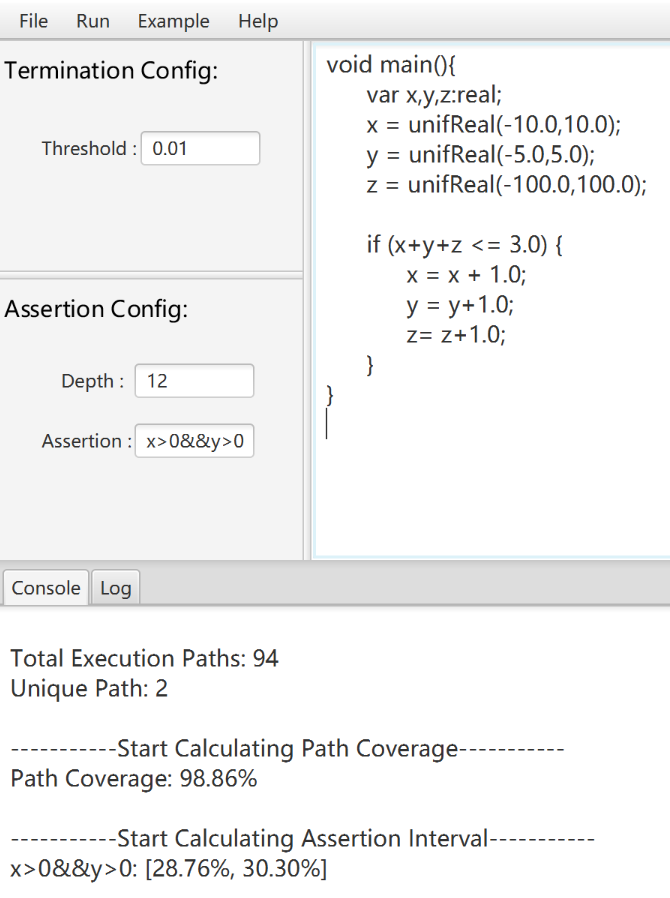
\includegraphics[scale=0.65]{img/interface2} 
		%\end{minipage}
	}
	\caption{PROPER User Interface} % %大图名称
	\label{interface} %图片引用标记
	%\setlength{\belowcaptionskip}{-1cm}   %调整图片标题与下文距离
\end{figure*}
The user interface is shown in Figure \ref{interface}. We show in (a) a running example of termination analysis, and in (b) a running example of assertion analysis. At the top of the interface is a row of menu bars, which are displayed in the form of pull lists. ``File" mainly includes functions of importing and saving files; ``Run" includes checking syntax, analyzing termination and analyzing assertion; ``Example" contains some built-in several examples, which can be directly executed. The concentration termination time can be set at the upper left of the interface; the recursion depth and assertion can be set at the lower left. Probabilistic programs can be written on the right. Alternatively, they can be  imported from external files. 

PROPER can deal with basic probabilistic programs with various structures, for which we have written a few simple but typical probabilistic programs, such as single while loop (eg. Simple), multiple nestings of while loops (eg. NestedLoop), conditions statement (if) in a while loop (eg. Tortoise-Hare), conditions-branch (if-else) in a while loop (eg. RandomWalk), nesting conditions statement in a while loop (eg. Bitcoin mining) and nesting conditions-branch statement in a while loop (eg. Gambler2). For loop guard related variables, we only support affine conditions, and for other variables, we can support the quadratic scenario of variable multiplication (eg. Car2). For the sake of understanding, we have shown some simple examples above. In addition, we also tried a large-scale program (eg.Herman), which generated 4935 constraints (linear equations) and 7561 parameters. These examples are available on \href{https://github.com/Healing1219/PROPER}{GitHub}.

Below we present some experimental results of analyzing probabilistic programs using PROPER. In Table~\ref{TerminationResult}, we display the experimental results about termination analysis, where $x_0$ means the initial value of each variable, $g(\ell_0,v_0)$ is the polynomial ranking supermartingale about the starting location, $UB(P)$ is the upper bound of expected termination time and $N$ is the bound that the probability of termination after $N$ steps shows an exponential decrement (we set the threshold to  be $0.01$). In order to read comfortably, we keep two decimal places by rounding.

\begin{table*}[htb]
	\centering
	\caption{Termination analysis}  
	\label{TerminationResult} 
	\begin{center}  
		\begin{tabular}{|l|l|l|l|l|}  
			\hline  	
			Example & $x_0$ & g($\ell_0,x_0$) & UB(P) & N\\ \hline  	
			Simple & $x=100$  & $6x$ & 601 & 1474.82 \\ \hline  		
			NestedLoop & $x=1, m=2$ & $1040\cdot m-1040\cdot x+208$ & 1249 & 158141.27 \\  \hline  
			Award & $bonus=0$ & $-4.0\cdot bonus+440$ & 441 &4522.28 \\  \hline  
			RandomWalk & $position=0$ & $-20\cdot position+120$ & 121 & 4695.66 \\  \hline  
			Gambler& $money=3$ & $400\cdot money+400$ & 1601 & 1506477.30 \\ \hline  		 
			Gambler2 & $money=10$ & $45.37 \cdot money+226.86$ & 908.44 & 3358.51 \\  \hline  
			Bitcoin mining & $coin=10$ & $5.32 \cdot coin$ & 54.18 & 6.39E7 \\  \hline 
			Tortoise-Hare & $h=5$, $t=30$ & $3\cdot t-3 \cdot h+27$ & 103 & 4264.27 \\  \hline  
			Cars & $s=0$, $s0=10$ & $1.90\!\cdot \!s0\!-\!1.90\! \cdot\! s\!+\!0.24\!\cdot\! s0^2\!+\!3.81$ & 47.67 & 165.90 \\	\hline 
			Cars2 & $s=0$, $s_0=10$ & \tabincell{c}{$3.05\cdot s_0-3.05 \cdot s+0.38\cdot s^2-$\\$0.76\cdot s\cdot s_0+0.38\cdot s_0^2+6.10$} & 75.67 & 259.12 \\  \hline 
			Herman & \tabincell{l}{$process_i=0$\\$(i=1\cdots 5)$,\\ $notStable=0$,\\$p=0.5$, $count=0$} & $-56\cdot notStable+280$ & 281 & 957.93 \\  \hline 
			Carton & \tabincell{l}{$total=0.0$\\ $nPacked=0$,\\$nPer=5$,$h=0$\\$count=0$,$l=0$} & \tabincell{c}{$45.31\cdot nPerCarton-$\\$45.31\cdot nPacked+45.31$} & 272.85 & 7878.55 \\  \hline 
		\end{tabular}  
	\end{center}  
\end{table*}

\begin{table*}[htb]
	\centering
	\caption{Estimating the probability intervals of assertions}
	\label{AssertionsResults} 
	\begin{tabular}{|m{55pt}<{\centering} |m{130pt}<{\centering} |m{50pt}<{\centering} |m{85pt}<{\centering}|}
		%{|c |c |c |c |}
		\hline  
		Example & Assertion &  $c$ & Bounds \\ \hline
		\iffalse
		\multirow{2}{*}{carton}
		& count$\geq$5 & 0.9485 & [0.948540, 1] \\ \cline{2-4}
		& count$\geq$10 & 0.9539, & [0.000639, 0.046711] \\ \cline{2-4}
		& count$\leq$7 & 0.9549 & [0.918762, 0.963832] \\ \cline{2-4}
		& totalWeight$\geq$5.5 & 0.9386 & [0.382145, 0.453010] \\ \cline{2-4}
		& totalWeight$\geq$6 & 0.9428 & [0.246186, 0.342997]  \\ \hline
		\multirow{2}{*}{herman}
		& $ count \geq 1$ & 0.9561 & [0.581128, 0.625000] \\ \cline{2-4}
		& $ count \geq 20$ & 0.9701 & [0.000000, 0.029876]  \\ \hline
		\fi
		\multirow{3}{*}{\makecell[c]{framingham}}
		& $points \geq 10$ & 96.36\% & [13.73\%, 17.36\%] \\ \cline{2-4}
		& $pointsErr-points \geq 5$ & 96.36\% & [77.81\%, 84.93\%]  \\ \cline{2-4}
		& $points-pointsErr \geq 5$ & 96.36\% & [17.76\%, 24.68\%]  \\ \hline
		\multirow{5}{*}{\makecell[c]{sum-three}}
		& $x>5 \ \&\& \ y>0$ & 98.86\% & [15.05\%, 16.36\%]  \\ \cline{2-4}
		&  \makecell[c]{$x>0 \ \&\&\ y>0 \&\& \ z>0$} & 98.86\% & [12.56\%, 13.73\%] \\ \cline{2-4}
		& $x+y>z+10$ & 98.86\% & [44.77\%, 47.07\%] \\ \cline{2-4}
		%		& $x+y+z>8$ & 0.9886 & [0.454482, 0.475890] \\ \cline{2-4}
		& $x+y+z>100$ & 98.86\% & [1.24\%, 2.59\%]  \\ \hline
		\iffalse
		\multirow{2}{*}{ckd-epi}
		& $f -f_1\geq0.1$ & 0.9252 & [0.351632, 0.426397] \\ \cline{2-4}
		& $f_1 -f\geq0.1$ & 0.9261 & [0.387275, 0.461157]  \\ \hline
		\fi
	\end{tabular}  
\end{table*}

The results of estimating the probability intervals of assertions as shown in Table~\ref{AssertionsResults} are consistent with those in~\cite{Sankaranarayanan2013Static}. A little difference lies in the syntax of assertions. We can support the conjunction operator  ``\&\&" in PROPER that is not available before. It can analyze situations where two or more conditions are met at the same time. In the table, an assertion is a Boolean expression; $c$ is the lower bound of path coverage; the column headed by Bounds gives the upper and lower bounds of the given assertions.

\section{Conclusion and Future Work}
Uncertainty exists in many software systems, including data analysis, stochastic algorithms and Monte Carlo simulation~\cite{HASTINGS1970Monte}. We have designed PROPER  to provide convenience and support for analyzing probabilistic programs.
PROPER is helpful to perform qualitative and quantitative analysis on the termination of probabilistic programs. It can also collect path sets with high confidence coverage and compute  probability intervals for assertions to hold in probabilistic programs.

\paragraph{Related tools}
Sofware tools for the analysis of probabilistic programs have not yet received much attention. 
As far as we know, the only existing tools are ProbFuzz~\cite{DBLP:conf/sigsoft/DuttaLHM18}, PSense~\cite{DBLP:conf/atva/HuangWM18} and PSI~\cite{DBLP:conf/cav/GehrMV16}.
PSI is a symbolic inference tool that approximates the probability density function represented by a probabilistic program. 
PSense is an automated verification tool that generates tight upper bounds for the sensitivity of probabilistic programs over initial inputs.
ProbFuzz is a tool for testing probabilistic programs. 
Both the aforementioned tools do not consider termination analysis of probabilistic programs. 
For example, ProbFuzz focuses on testing rather than verification of probabilistic programs, 
PSI considers only inference and PSense solves sensitivity instead. 
Moreover, PSI/PSense requires that the input probabilistic while loop has a bounded number of loop iterations, while we can handle probabilistic loops with an unbounded number of loop iterations.

Furthermore, our tool compares with the other three tools (i.e., the tools implemented for~\cite{Sankaranarayanan2013Static}, \cite{Ngo2018Bounded} and \cite{J2019Computing}) and has different strengths.The tool for \cite{Sankaranarayanan2013Static} can prove almost-sure termination of probabilistic programs, but cannot generate an upper bound for the expected termination time as our tool can do; the tool for \cite{Ngo2018Bounded} generates upper bounds for expected cost consumption, but its algorithm is not complete for linear ranking super-martingales since it is not based on Farkas' Lemma while our algorithm is complete; the tool for \cite{J2019Computing} aims at a sound and complete algorithm for deriving expected runtime, but can only handle a special class of affine programs where the loop guard contains only one linear inequality and the loop body is simply a probabilistic choice of incremental assignments of the form $x:=x+c$ where $x$ is a program variable and $c$ is a constant, while our algorithm aims at general affine probabilistic programs. 

\paragraph{Fugure work}
Admittedly, we have only solved some aspects of the complex problem of probabilistic program analysis and verification. There are still many ways to improve the tool.
\begin{enumerate}
	\item Currently, PROPER only deals with linear programs. That is, it cannot handle variable multiplication, division and exponents, etc., regardless of the termination analysis or the estimation of assertion probability intervals.
	\item Non-deterministic probabilistic programs  are also not supported. PROPER requires the behavior of the input program to be fully probabilistic, and there is no non-deterministic transitions. 
	\item In the future, we hope to find a better way to compute accurate termination time and probability intervals under the premise of ensuring high efficiency. 
\end{enumerate}

\begin{thebibliography}{00}
\bibitem{Arora1998Proof}
Arora, S., Lund, C., Motwani, R., Sudan, M., Szegedy, M., Proof verification and the hardness of approximation problems. Journal of the ACM \textbf{45}(3), 501--555 (1998).
\bibitem{Azuma1967}
Azuma, K., Weighted sums of certain dependent random variables. Tohoku Mathematical Journal \textbf{19}(3), 357--367 (2010).
\bibitem{Bennett1962}
Bennett G., Probability Inequalities for the Sum of Independent Random Variables. Journal of the American Statistical Association \textbf{57}(297), 33--45 (1962).
\bibitem{Chakarov2013Martingales}
Chakarov A., Sankaranarayanan S., Probabilistic Program Analysis with Martingales. In: CAV, pp. 511--526  (2013).
\bibitem{kris2016termination}
Chatterjee, K., Fu, H., Goharshady, A.K., Termination Analysis of Probabilistic Programs through Positivstellensatz's. In: CAV, pp. 3--22 (2016). doi{10.1007/978-3-319-41528-4\_1 }.
\bibitem{cha2015algorithmic}
Chatterjee, K., Fu, H., Novotn\'{y}, P., Hasheminezhad, R., Algorithmic analysis of
qualitative and quantitative termination problems for affine probabilistic programs. In: POPL, pp. 327--342 (2016).
\bibitem{DBLP:conf/sigsoft/DuttaLHM18}
Dutta S., Legunsen O., Huang Z., et al., Testing probabilistic programming systems. In: FSE, pp. 574--586 (2018). doi{10.1145/3236024.3236057}.
\bibitem{Hermanns2013Probabilistic}
Fioriti, L.M.F., Hermanns, H., Probabilistic termination : Soundness, completeness, and compositionality. In: POPL, pp. 489--501 ACM (2015).
\bibitem{DBLP:conf/cav/GehrMV16}
Gehr, T., Misailovic, S., Vechev, M., {PSI:} Exact Symbolic Inference for Probabilistic Programs. In: CAV, pp. 62--83 (2016). doi{10.1007/978-3-319-41528-4\_4}.
\bibitem{Geldenhuys2012symbolic}
Geldenhuys, J.,Dwyer M. B., Visser W., Probabilistic symbolic execution. In: ISSTA, pp. 166--176 ACM(2012).
\bibitem{Noah2012language}
Goodman, N., Mansinghka, V., Roy, D., Bonawitz, K., Tarlow, D., Church: a language for generative models. In: UAI, pp. 220--229. AUAI Press (2012).
\bibitem{Noah2014language}
Goodman, N., Stuhlmüller A., The Design and Implementation of Probabilistic Programming Languages. http://dippl.org.  (2014).
\bibitem{Handelman1988}
Handelman, D., Representing polynomials by positive linear functions on compact convex polyhedras. Pacific J. Math \textbf{132}, 35--62 (1988).
\bibitem{HASTINGS1970Monte}
Hastings, W., Monte Carlo sampling methods using Markov chains and their applications. Journal of the ACM, 97--109 (1970).
\bibitem{Bingsheng2020}
He, B., Ma F., Yuan X., Optimally linearizing the alternating direction method of multipliers for convex programming. Computational Optimization and Applications \textbf{75}, 361--388 (2020).
\bibitem{Hoeffding1963}
Hoeffding W., Probability Inequalities for Sums of Bounded Random Variables. Journal of the American Statistical Association \textbf{58} (301), 13--30 (1963).
\bibitem{DBLP:conf/atva/HuangWM18}
Huang Z., Wang Z., Misailovic S., PSense: Automatic Sensitivity Analysis for Probabilistic Programs. In: ATVA, pp. 387--403 (2018). 
\bibitem{J2019Computing}
Jürgen Giesl, Giesl P., Hark M., Computing Expected Runtimes for Constant Probability Programs.Automated Deduction – CADE 27(2019).
\bibitem{McDiarmid1998Concentration}
McDiarmid C., Concentration. In Probabilistic Methods for Algorithmic Discrete Mathematics. Algorithms in combinatorics \textbf{16}, 195--248 (1998).
\bibitem{Ngo2018Bounded}
Ngo V C , Carbonneaux Q , Hoffmann J., Bounded Expectations: Resource Analysis for Probabilistic Programs.Programming Language Design \& Implementatio,496--512(2018).
\bibitem{Sankaranarayanan2013Static}
Sankaranarayanan, S., Chakarov, A., Gulwani, S., Static Analysis for Probabilistic Programs: Inferring Whole Program Properties from Finitely Many Paths. ACM SIGPLAN Notices \textbf{48}(6), 447--458 (2013).
\bibitem{Dav2016Design}
Tolpin, D., Willem, V. D. M. J., Yang, H., Wood, F., Design and Implementation of Probabilistic Programming Language Anglican. In: IFL, 6:1–6:12. (2016).
\bibitem{tran2016edward}
Tran, D., Kucukelbir, A., Dieng, A. B., Rudolph, M., Liang, D., Blei, D. M., Edward, A library for probabilistic modeling, inference, and criticism. (2016) doi{1610.09787}.
\bibitem{Visser2012Green}
Visser, W., Geldenhuys, J. , Dwyer, M. B., Green: reducing, reusing and recycling constraints in program analysis. In: FSE, pp. 1--11 (2012).
\end{thebibliography}
\end{document}
